\documentclass[11pt,border=2mm]{standalone}
\usepackage{csquotes}
\usepackage[backend=biber,style=numeric,sorting=none]{biblatex}

\providecommand{\FigScale}{1}

\usepackage{tikz}
\usetikzlibrary{arrows.meta, calc}

% ---- colours ----
\definecolor{IBM1}{HTML}{648fff}      % annotation blue
\definecolor{traceFill}{HTML}{C9D6F0} % light-blue trace fill
\definecolor{traceEdge}{HTML}{6E6E76} % grey trace outline
\definecolor{dotCol}{HTML}{3C3C42}    % dotted centre line

\begin{document}
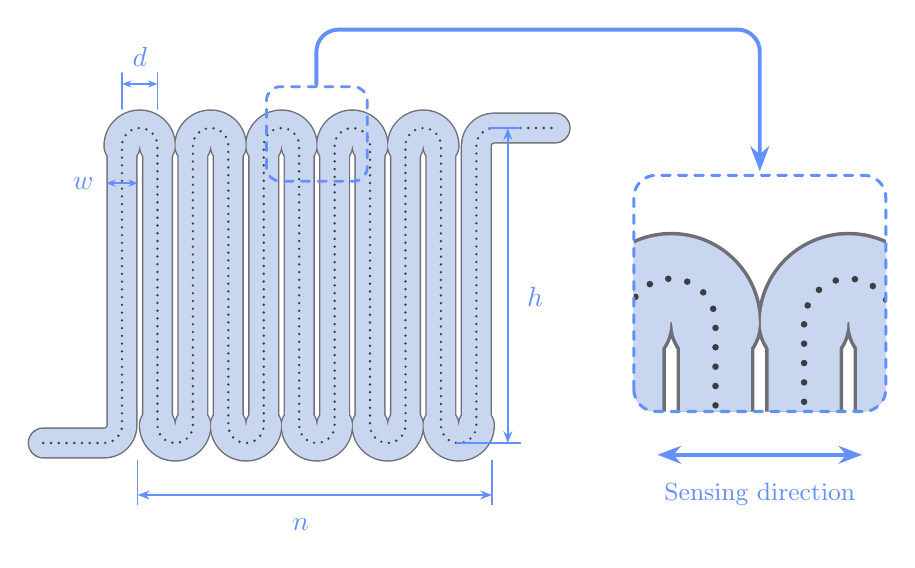
\begin{tikzpicture}[scale=\FigScale, line cap=round, line join=round]

\def\fingW{0.36}
\def\turnW{0.44}
\def\edge{0.018}

\pgfmathsetmacro{\fingWout}{\fingW+2*\edge}
\pgfmathsetmacro{\turnWout}{\turnW+2*\edge}
\def\turnR{0.225}
\def\dotW{0.95}

\def\meander{%
 (-1.0,0) -- (0,0) --
 (0,4) -- (0.45,4) -- (0.45,0) -- (0.9,0) --
 (0.9,4) -- (1.35,4) -- (1.35,0) -- (1.8,0) --
 (1.8,4) -- (2.25,4) -- (2.25,0) -- (2.7,0) --
 (2.7,4) -- (3.15,4) -- (3.15,0) -- (3.6,0) --
 (3.6,4) -- (4.05,4) -- (4.05,0) -- (4.5,0) --
 (4.5,4) -- (5.5,4)%
}

\def\topturns{0,0.9,1.8,2.7,3.6}
\def\botturns{0.45,1.35,2.25,3.15,4.05}

\newcommand{\drawtrace}{%
  \draw[traceEdge, line width=\fingWout cm, rounded corners=\turnR cm] \meander;
  \foreach \x in \topturns {\draw[traceEdge, line width=\turnWout cm]
          (\x,3.775) arc[start angle=180,end angle=0,radius=\turnR];}
  \foreach \x in \botturns {\draw[traceEdge, line width=\turnWout cm]
          (\x,0.225) arc[start angle=180,end angle=360,radius=\turnR];}
  \draw[traceFill, line width=\fingW cm, rounded corners=\turnR cm] \meander;
  \foreach \x in \topturns {\draw[traceFill, line width=\turnW cm]
          (\x,3.775) arc[start angle=180,end angle=0,radius=\turnR];}
  \foreach \x in \botturns {\draw[traceFill, line width=\turnW cm]
          (\x,0.225) arc[start angle=180,end angle=360,radius=\turnR];}
  \draw[dotCol, line width=\dotW pt, dash pattern=on 0pt off 2.8pt,
        rounded corners=\turnR cm] \meander;%
}

\def\zx{2.475}
\def\zy{3.925}
\def\zmag{2.5}
\pgfmathsetmacro{\zhw}{1.6/\zmag}   \pgfmathsetmacro{\zhh}{1.5/\zmag}
\pgfmathsetmacro{\zboxL}{\zx-\zhw}  \pgfmathsetmacro{\zboxR}{\zx+\zhw}
\pgfmathsetmacro{\zboxB}{\zy-\zhh}  \pgfmathsetmacro{\zboxT}{\zy+\zhh}

\drawtrace

\tikzset{
  dimline/.style={IBM1, line width=0.7pt,
                  {Stealth[length=1.5mm]}-{Stealth[length=1.5mm]}},
  dimtiny/.style={IBM1, line width=0.7pt,
                  {Stealth[length=1.2mm]}-{Stealth[length=1.2mm]}},
  extline/.style={IBM1, line width=0.5pt},
}

% d
\draw[extline] (0,4.24) -- (0,4.7);
\draw[extline] (0.45,4.24) -- (0.45,4.7);
\draw[dimtiny] (0,4.56) -- (0.45,4.56);
\node[IBM1] at (0.225,4.9) {$d$};

% w
\draw[dimtiny] (-0.2,3.3) -- (0.2,3.3);
\node[IBM1, anchor=east] at (-0.24,3.3) {$w$};

% h
\draw[extline] (4.25,0) -- (5.06,0);
\draw[extline] (4.66,4) -- (5.06,4);
\draw[dimline] (4.9,0) -- (4.9,4);
\node[IBM1, anchor=west] at (5.02,1.85) {$h$};

% n
\draw[extline] (0.2,-0.22) -- (0.2,-0.78);
\draw[extline] (4.7,-0.22) -- (4.7,-0.78);
\draw[dimline] (0.2,-0.66) -- (4.7,-0.66);
\node[IBM1] at (2.27,-1.04) {$n$};

\draw[IBM1, line width=1.0pt, dashed, rounded corners=5pt]
      (\zboxL,\zboxB) rectangle (\zboxR,\zboxT);

\draw[IBM1, line width=1.4pt, rounded corners=8pt, -{Stealth[length=3.2mm]}]
      (2.469,4.55) -- (2.469,5.25) -- (8.1,5.25) -- (8.1,3.45);

\begin{scope}
  \clip[rounded corners=8pt] (6.5,0.4) rectangle (9.7,3.4);
  \begin{scope}[transform canvas={shift={(8.1,1.9)},scale=\zmag,shift={(-\zx,-\zy)}}]
    \drawtrace
  \end{scope}
\end{scope}
\draw[IBM1, line width=1.1pt, dashed, rounded corners=8pt]
      (6.5,0.4) rectangle (9.7,3.4);

\draw[IBM1, line width=1.5pt, {Stealth[length=3mm]}-{Stealth[length=3mm]}]
      (6.8,-0.15) -- (9.4,-0.15);
\node[IBM1, font=\small] at (8.1,-0.65) {Sensing direction};

\end{tikzpicture}
\end{document}
